% Theoretical background
%\clearpage%if the chapter heading starts close to bottom of the page, force a
% line break and remove the vertical vspace
\vspace{21.5pt}
\chapter{Design, Implementations and Results}

This chapter outlines the methodology applied in designing and implementing
file fuzzer integration with a target program, which interprets inputs from
files within the Zephyr RTOS. This program, being one of the samples in
Zephyr RTOS\cite{Security75:online}, has been chosen to underscore the
practical relevance of this study.

While various fuzzers have been discussed in the preceding sections,
AFL++\cite{257204} and libFuzzer\cite{libFuzze17:online} have been selected for demonstration due to their distinct
capabilities and widespread usage. These fuzzers serve to emphasize the
significance of the study, considering the prevalent application of
real-time operating systems in modern embedded devices.

The fuzzing tests have been conducted on a Linux system,
where AFL++\cite{257204} and libFuzzer\cite{libFuzze17:online} have already been installed, and the Zephyr RTOS environment has been set up.

\section{Implementations Using AFL++}
This section delineates the detailed steps for setting up the
AFL++\cite{257204} fuzzer using a Docker\cite{anderson2015docker}
container and compiling the target program.

The selection of the AFL++ Docker image as the basis for the initial setup was
driven by the recommendations provided by the AFL++ documentation. This particular
image is endorsed due to its comprehensive inclusion of all necessary AFL++ tools,
consolidated in a singular location, thereby facilitating a streamlined
and efficient setup process\cite{257204}.

Steps to start fuzzing with AFL++:

\subsection*{Step 1: Docker Script for AFL++}
The first step involves pulling the AFL++ Docker image and running a container:
\begin{minted}[linenos,frame=lines,baselinestretch=1.2,breaklines]{sh}
#!/bin/bash
# Pull the AFL++ Docker image
$ docker pull aflplusplus/aflplusplus
# Run a container using the pulled image
$ docker run -ti -v /home/uname:/home/uname --name afl_container aflplusplus/aflplusplus
# Get into the container
$ docker exec -it afl_container /bin/bash
\end{minted}

This script facilitates the deployment of the AFL++ fuzzer in a Docker container,
streamlining the setup process for fuzzing tests.

\subsection*{Step 2: List of Files}
The relevant files for the next step are:
\begin{itemize}
    \item \texttt{main.c}: The target program in appendix-\ref{appx:first}.
    \item \texttt{CMakeLists.txt}: Build configuration file.
\end{itemize}

The detailed implementation of the target program can be
found in Appendix-\ref{appx:first}. This program, written
in C, exemplifies the integration of fuzz testing in a Zephyr RTOS environment.

\subsection*{Explanation of the Main Program:}
The \texttt{main.c} program serves as the target for the fuzz testing,
designed to illustrate potential vulnerabilities within the Zephyr RTOS.
It's structured to simulate a scenario where specific inputs could trigger a
failure case, providing a practical example for the fuzzing tests conducted.

This particular program was chosen due to its inherent characteristics that
are pivotal for fuzz testing. Fuzz testing is coverage-based and necessitates
the concealment of a failure point— in this instance, a write through a null
pointer—deep within the call structure of the program. While such a concealed
failure is typically challenging to uncover with randomly-selected input,
a fuzzer is designed to locate it in a relatively linear time by systematically
exploring each function.

Even in scenarios characterized by a low probability of discovering the failure,
as in 1 in \(2^{56}\), which conventionally demands extensive computational
time and resources, the fuzzer is capable of identifying the vulnerability in
approximately 20 seconds. This efficiency is attributed to the distinct
testability of each code segment, necessitating the generation of specific
handler functions and the deactivation of certain optimizations.

The program contains several key components:

\begin{itemize}
\item \textbf{global\_null\_ptr}: A pointer that, under certain conditions,
can be triggered to write through a null, simulating a failure.
\item \textbf{key Array and found Array}: These arrays are used to check against
the input data and keep track of discovered keys.
\item \textbf{GEN\_CHECK Macro}: This macro generates a series of check
functions that recursively call each other to simulate a deep call tree.
\end{itemize}

Upon execution, the program reads input data from a file. It then processes
this data through the series of check functions generated by
the \texttt{GEN\_CHECK} macro. If a match with the key array is found,
it simulates a failure by attempting a write through the \texttt{global\_null\_ptr}.
The failure case is hidden deep within the call tree, making it difficult to
discover through random inputs but still discoverable through fuzz testing.

For a more detailed view of the \texttt{main.c} file, refer to
Appendix-\ref{appx:first}.

\textbf{Explanation of the CMakeLists.txt:}
The \texttt{CMakeLists.txt} file is used for configuring the build system
of the \texttt{sample\_zephyr\_afl} project in the zephyr RTOS. Here is an
explanation of its components:

\begin{itemize}
    \item \texttt{cmake\_minimum\_required(VERSION 3.20.0)}: This command
    specifies the minimum version of CMake that is required, which is version
    3.20.0 in this case.
    \item \texttt{project(sample\_zephyr\_afl)}: This command sets the name
    of the project to \texttt{sample\_zephyr\_afl}.
    \item \texttt{option(USE\_AFL "Use afl" OFF)}: This command declares an
    option named \texttt{USE\_AFL} that determines whether to use AFL. It is
    set to \texttt{OFF} by default.
    \item The conditional block \texttt{if(USE\_AFL)} checks
    whether \texttt{USE\_AFL} is turned on. If it is, the compiler is
    set to \texttt{afl-gcc-fast}\cite{AFLplusp13:online}, and additional
    compiler flags for coverage are added. If \texttt{USE\_AFL} is turned off,
    the compiler is set to \texttt{gcc}\cite{GCCtheGN9:online}.
    \item \texttt{add\_executable(zephyr\_aflfuzzer src/main.c)}: This
    command specifies that an executable named \texttt{zephyr\_aflfuzzer}
    should be created from the source file \texttt{src/main.c}.
\end{itemize}

For a more detailed view of the \texttt{CMakeLists.txt} file, refer to
Appendix-\ref{appx:first}.

\subsection*{Step 3: Build and Compile}
A new directory, \texttt{build}, is created to contain all the build files.
The \texttt{cmake} command is invoked with the \texttt{-DUSE\_AFL=ON} option,
indicating that the build should be configured to
use \texttt{afl-gcc-fast}\cite{AFLplusp13:online}.

\begin{minted}[linenos,frame=lines,baselinestretch=1.2,breaklines]{sh}
    $ mkdir build
    $ cd build
    $ cmake -DUSE_AFL=ON ..
    $ make
\end{minted}

\subsection*{Step 4: Valid Input for the Target}
A binary file is created with a specific sequence of bytes.
This file will serve as the initial and valid input or corpus for the fuzzer,
allowing it to explore different code paths.

\begin{minted}{sh}
    $ echo -n -e '\x9e\x21\x0c\x18\x9d\xd1\x7e' > input_data/test_data.bin
\end{minted}

\subsection*{Step 5: Testing, Results, Analysis and Report}
AFL++ is invoked with the \texttt{afl\-fuzz} command inside the docker container,
specifying the input directory containing the corpus \texttt{input\_data} and
the output directory \texttt{output}. The built binary \texttt{zephyr\_aflfuzzer}
is then executed with AFL++'s syntax for specifying input files.

\begin{minted}{sh}
    $ afl-fuzz -i input_data/ -o output/ -- ./sample_zephyr_afl/build/zephyr_aflfuzzer @@
\end{minted}

This section breaks down the components of this command\cite{257204}:

\begin{itemize}
    \item \texttt{afl-fuzz}: This is the command to initiate the AFL++ fuzzer.
    \item \texttt{-i input\_data/}: The \texttt{-i} flag specifies the
    input directory containing the `corpus' of sample input files,
    which serve as a basis to generate new test cases.
    \item \texttt{-o output/}: The \texttt{-o} flag denotes the output
    directory where AFL stores the results of the fuzzing session,
    including any crashes or hangs it discovers.
    \item \texttt{--}: This symbol denotes the end of the options passed
    to the AFL fuzzer. Any parameter listed after this is considered as
    an argument to the program being fuzzed, not as an option to AFL.
    \item \texttt{./sample\_zephyr\_afl/build/zephyr\_aflfuzzer}: This is the
    path to the target binary that will be fuzzed by AFL.
    \item \texttt{@@}: This placeholder is replaced by AFL with the name of a
    file containing the test case each time the target binary is run,
    allowing AFL to run the program with a multitude of different inputs
    without needing to modify the command line each time.
\end{itemize}

The Figure-\ref{fig:afl_execute_1} shows the AFL++ execution screen.
\begin{figure}[H]
        \adjustbox{width=\textwidth}{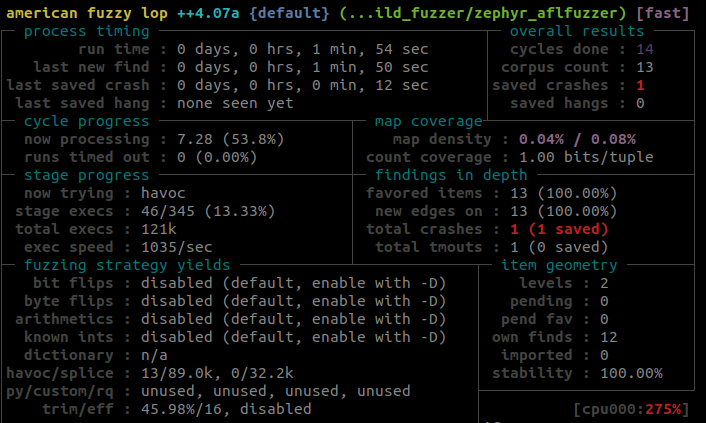
\includegraphics{afl_execute_1}}
        \caption{AFL++ Execution Screen}\label{fig:afl_execute_1}
\end{figure}

Important elements of the user interface shown below\cite{257204}:

\begin{itemize}
    \item \textbf{process\_timing:} This section shows how long the fuzzer has
    been running and the current time.
    \item \textbf{stage progress:} Here, AFL++ displays the progress of the
    current fuzzing stage in terms of execution and the total number of inputs
    to be tested in this stage.
    \item \textbf{findings in depth:} This area provides details about the paths
    discovered, including the number of unique crashes, hangs, and paths found
    during the fuzzing session.
    % \item \textbf{fuzzing strategy yields:} This section gives insights into the
    % effectiveness of various fuzzing strategies by showing how many new paths, crashes, or hangs each strategy has yielded.
    \item \textbf{item geometry:} This displays information related to the paths
    taken through the program, such as the depth and width of the explored paths.
    %\item \textbf{pending favs:} It shows the number of favored paths (interesting inputs) that are yet to be processed.
    %\item \textbf{map coverage:} This section gives a snapshot of the code coverage, indicating the percentage of the target's codebase that has been executed by the inputs generated so far.
    %\item \textbf{speed:} This denotes the execution speed of the fuzzer, typically represented in executions per second.
    %\item \textbf{cycle progress:} This shows the progress of the current fuzzing cycle, indicating how much of the input corpus has been processed in this cycle.
    %\item \textbf{total execs:} This is a count of the total number of input cases that AFL++ has executed since the start of the fuzzing session.
    %\item \textbf{exec reliability:} This metric shows the reliability of the execution, highlighting if any executions were aborted.
    %\item \textbf{exec stability:} This indicates the stability of the target program during fuzzing, represented as a percentage.
    %\item \textbf{has\_new\_finds:} This field will be highlighted if AFL++ has found new, unique crashes or paths since the last UI update.
    %\item \textbf{has\_uniq\_finds:} This will be highlighted if AFL++ has found any new unique crashes, hangs, or paths since the last UI update.
    %\item \textbf{command:} At the bottom of the screen, the exact command-line used to start AFL++ is displayed.
\end{itemize}

As depicted in Figure-\ref{fig:afl_execute_1}, the binary generated
(as detailed in Appendix-1) resulted in AFL++ creating a total of
13 corpus and identifying one crash. Remarkably, a scenario with a
probability of \(1\) in \(2^{56}\), which would traditionally
require several months to years of computation in a large datacenter,
was resolved by the fuzzer in under two minutes.

The resulting outputs are stored in the \textit{output} directory.
The coverage report of the execution can be generated using \textit{afl-cov}\cite{GitHubmr91:online}.
The corresponding command is as follows:

\begin{minted}{sh}
    $ afl-cov -d output/ --coverage-cmd "./sample_zephyr_afl/build/zephyr_aflfuzzer @@" --code-dir ./sample_zephyr_afl/
\end{minted}

The Figure-\ref{fig:afl_cov} shows the \texttt{afl-cov} report of the execution.
\begin{figure}[H]
        \adjustbox{width=\textwidth}{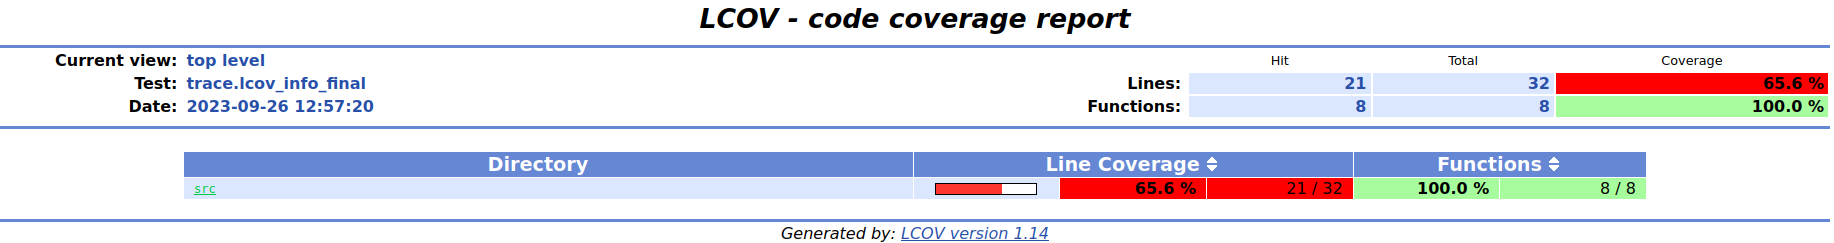
\includegraphics{afl_cov}}
        \caption{LCOV Coverage Report\cite{UbuntuMa97:online}}\label{fig:afl_cov}
\end{figure}

AFL++ includes a visualization tool called \texttt{afl-plot}\cite{AFLFunct92:online},
which is instrumental in assessing the performance of fuzzing campaigns.
This tool generates a series of graphs that provide insights into several
crucial metrics throughout the fuzzing process. These metrics include,
but are not limited to, the number of crashes discovered,
the speed of execution, and the progression of path discovery over time.

\begin{minted}{sh}
    $ afl-plot output/default/ output/output_plot/
\end{minted}

The Figure-\ref{fig:afl_plot} shows the \texttt{afl-plot} report of the execution.
\begin{figure}[H]
        \adjustbox{width=\textwidth}{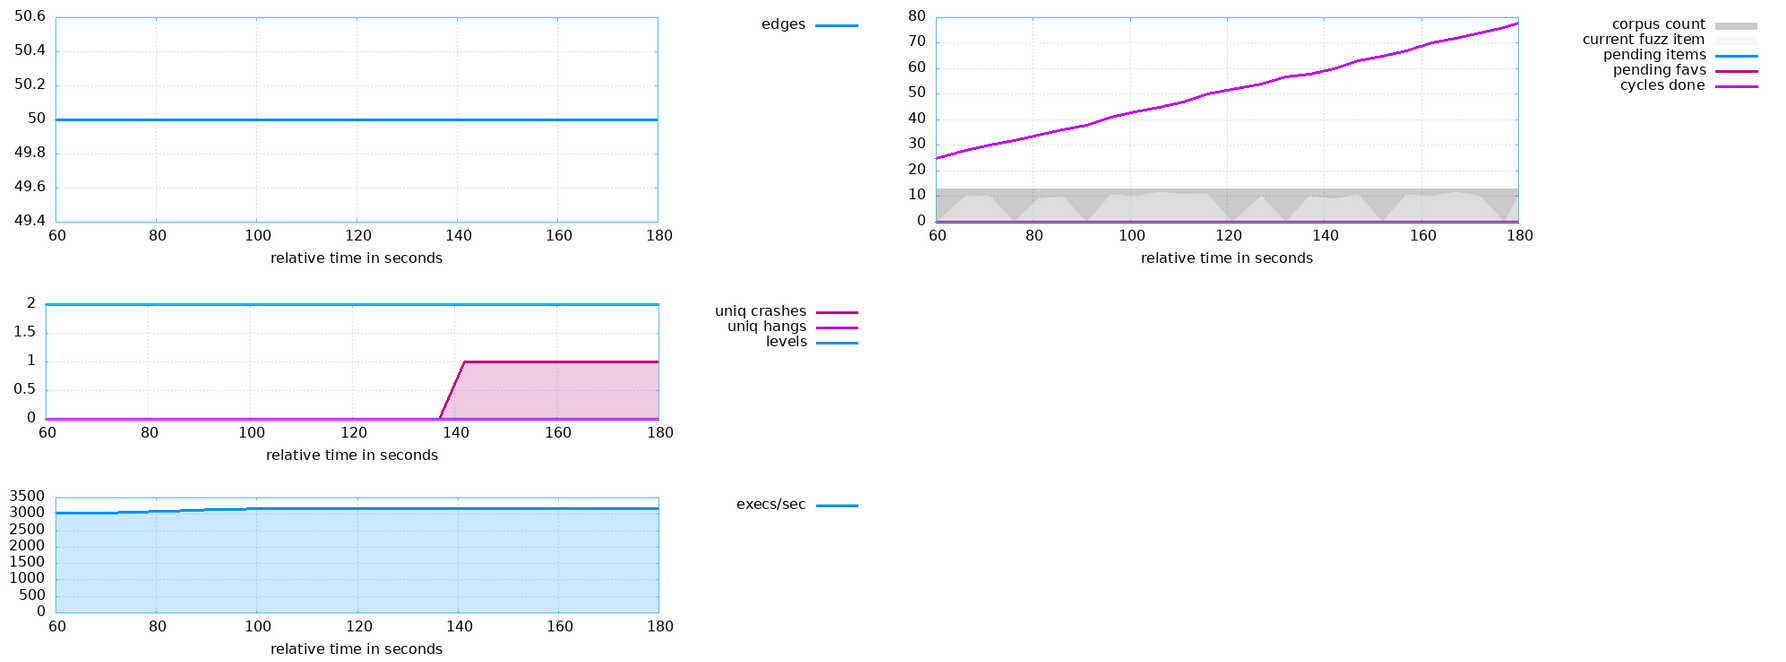
\includegraphics{afl_plot}}
        \caption{\texttt{afl-plot} Report}\label{fig:afl_plot}
\end{figure}

The fuzzing tests adeptly illustrate the utilization of the AFL++ fuzzer,
accompanied by tools such as afl-cov and afl-plot, highlighting
the vulnerabilities that can be unearthed, alongside generating
comprehensive coverage and graphical representations. This proof of
concept underscores the potency of employing fuzzing with AFL++,
demonstrating its utility in uncovering concealed vulnerabilities
and enhancing system robustness.

The AFL++ fuzzer, renowned for its efficiency and effectiveness,
exemplifies its capability to discern vulnerabilities, even those
embedded deep within the code structure, in a remarkably truncated timeframe.
The accompanying tools, afl-cov and afl-plot, augment this process
by providing detailed coverage reports and graphical data, thereby
facilitating a more nuanced understanding of the system's susceptibility
to potential threats. The insights derived from this study illuminate the
myriad possibilities and benefits of integrating AFL++ into the development
cycle, underscoring its potential contribution to fortifying system security.

\section{Implementations Using libFuzzer}
LibFuzzer\cite{libFuzze17:online}, an integral part of the LLVM Compiler\cite{libFuzze42:online} Infrastructure,
is chosen for this Proof of Concept (PoC) due to its distinct attributes and capabilities.
LibFuzzer is renowned for its efficiency in performing coverage-guided fuzzing,
which is instrumental in identifying hidden vulnerabilities within a system\cite{fuzzingt51:online}.

The fuzzer's seamless integration with the Clang compiler\cite{ClangCLa81:online} and its capability
to perform in-memory fuzzing make it a valuable tool in assessing the security
and robustness of software systems.

Steps to start fuzzing with libFuzzer:

\subsection*{Step 1: Setting up Environment}
To set up the necessary environment, a Linux-based operating system,
specifically Ubuntu, is utilized. Furthermore, the installation of a recent
version of the Clang compiler is requisite for the successful execution of the
libFuzzer\cite{ClangCLa81:online}.

\subsection*{Step 2: List of Files}
The relevant files for the next step are:
\begin{itemize}
    \item \texttt{main.c}: The target program in Appendix-\ref{appx:second}.
    \item \texttt{CMakeLists.txt}: Build configuration file.
\end{itemize}

The detailed implementation of the target program can be
found in Appendix-\ref{appx:second}.

Comparing this program in Appendix-\ref{appx:second} to the one utilized for
AFL++ in Appendix-\ref{appx:first}, there are fundamental differences that
can be highlighted:

This is a simple example of fuzz test integration with Zephyr apps
that displays LLVM libfuzzer's most important feature: it's ability to
detect and explore deep and complicated call trees by exploiting
coverage information gleaned from instrumented binaries.

\begin{itemize}
    \item \textbf{Entry Point:} In the context of libFuzzer, the program uses a function
    named \texttt{LLVMFuzzerTestOneInput} as the entry point,
    which is specifically designed for integration with libFuzzer.
    This contrasts with the AFL++ target program, where the
    \texttt{main} function serves as the entry point.
    \item \textbf{Input Handling:} The libFuzzer target program directly uses
    the input data provided to the \texttt{LLVMFuzzerTestOneInput} function,
    representing a more straightforward handling of input compared to the
    AFL++ target program, which might necessitate additional steps for input
    retrieval and processing.
\end{itemize}

\textbf{Explanation of the CMakeLists.txt:}
The \texttt{CMakeLists.txt} file is used for configuring the build system
of the \texttt{sample\_zephyr\_libFuzzer} project in the zephyr RTOS.
Here is an explanation of its components:

\begin{itemize}
    \item \texttt{cmake\_minimum\_required(VERSION 3.20.0)}: Specifies the minimum required version of CMake to be 3.20.0.

    \item \texttt{project(sample\_zephyr\_libfuzzer)}: Names the project as \texttt{sample\_zephyr\_libfuzzer}.

    \item \texttt{option(USE\_LIBFUZZER "Build with libfuzzer" OFF)}: Declares an option \texttt{USE\_LIBFUZZER}, which is turned OFF by default but can be set to ON to enable building with libFuzzer.

    \item \texttt{set(CMAKE\_C\_COMPILER clang)}: Sets the C compiler for the project to Clang.

    \item \texttt{if(USE\_LIBFUZZER)}: Checks if \texttt{USE\_LIBFUZZER} is enabled.

    \begin{itemize}
        \item \texttt{add\_definitions(-DUSE\_LIBFUZZER)}: Adds a definition for \texttt{USE\_LIBFUZZER} for the preprocessor.

        \item \texttt{set(CMAKE\_C\_FLAGS "... -fsanitize=fuzzer,address,undefined")}: Sets the compiler flags to enable sanitizers and fuzzer.

        \item \texttt{set(CMAKE\_EXE\_LINKER\_FLAGS "... -fsanitize=fuzzer,address,undefined")}: Sets the linker flags to enable sanitizers and fuzzer.

        \item \texttt{set(CMAKE\_C\_FLAGS "... -fprofile-instr-generate -fcoverage-mapping")}: Enables flags for generating profile instrumentation and coverage mapping.
    \end{itemize}

    \item \texttt{add\_executable(zephyr\_libfuzzer src/main.c)}: Defines an executable target named \texttt{zephyr\_libfuzzer} from the source file \texttt{src/main.c}.

    \item \texttt{if(USE\_LIBFUZZER)}: If \texttt{USE\_LIBFUZZER} is enabled, sets additional linker flags for the target \texttt{zephyr\_libfuzzer} to enable the necessary sanitizers for fuzzing.
\end{itemize}

\subsection*{Step 3: Build and Compile}
A new directory, \texttt{build}, is created to contain all the build files.
The \texttt{cmake} command is invoked with the \texttt{-DUSE\_LIBFUZZER=ON} option,
indicating that the build should be configured to
use \texttt{clang}\cite{ClangCLa81:online}.

\begin{minted}[linenos,frame=lines,baselinestretch=1.2,breaklines]{sh}
    $ mkdir build
    $ cd build_fuzzer
    $ cmake -DUSE_LIBFUZZER=ON ..
    $ make
    $ ./zephyr_libfuzzer
\end{minted}

\subsection*{Step 4: Testing, Results and Analysis}
The CMake configuration for the \texttt{sample\_zephyr\_libfuzzer} project sets
a robust foundation for enabling fuzz testing with \texttt{libFuzzer} and
Clang's sanitizers. The flexibility to toggle the \texttt{libFuzzer} integration
is an essential attribute, as it allows the program to be compiled with or
without the fuzzing infrastructure. When the \texttt{USE\_LIBFUZZER} option is
activated, the system adeptly applies the necessary compiler and linker flags
to incorporate \texttt{libFuzzer}, address sanitizer, and undefined behavior
sanitizer. The added instrumentation flags for profile generation and coverage
mapping suggest that the project not only focuses on uncovering vulnerabilities
but also on gauging the coverage of the testing process. This kind of approach
ensures a two-fold outcome: vulnerability discovery and code execution
coverage analysis. Ultimately, it provides a comprehensive insight into the
robustness against arbitrary and malicious inputs, rendering a pivotal report
on its security stature.


The Figure-\ref{fig:lib_fuzzer} shows the libFuzzer execution output.
\begin{figure}[H]
    \adjustbox{width=\textwidth}{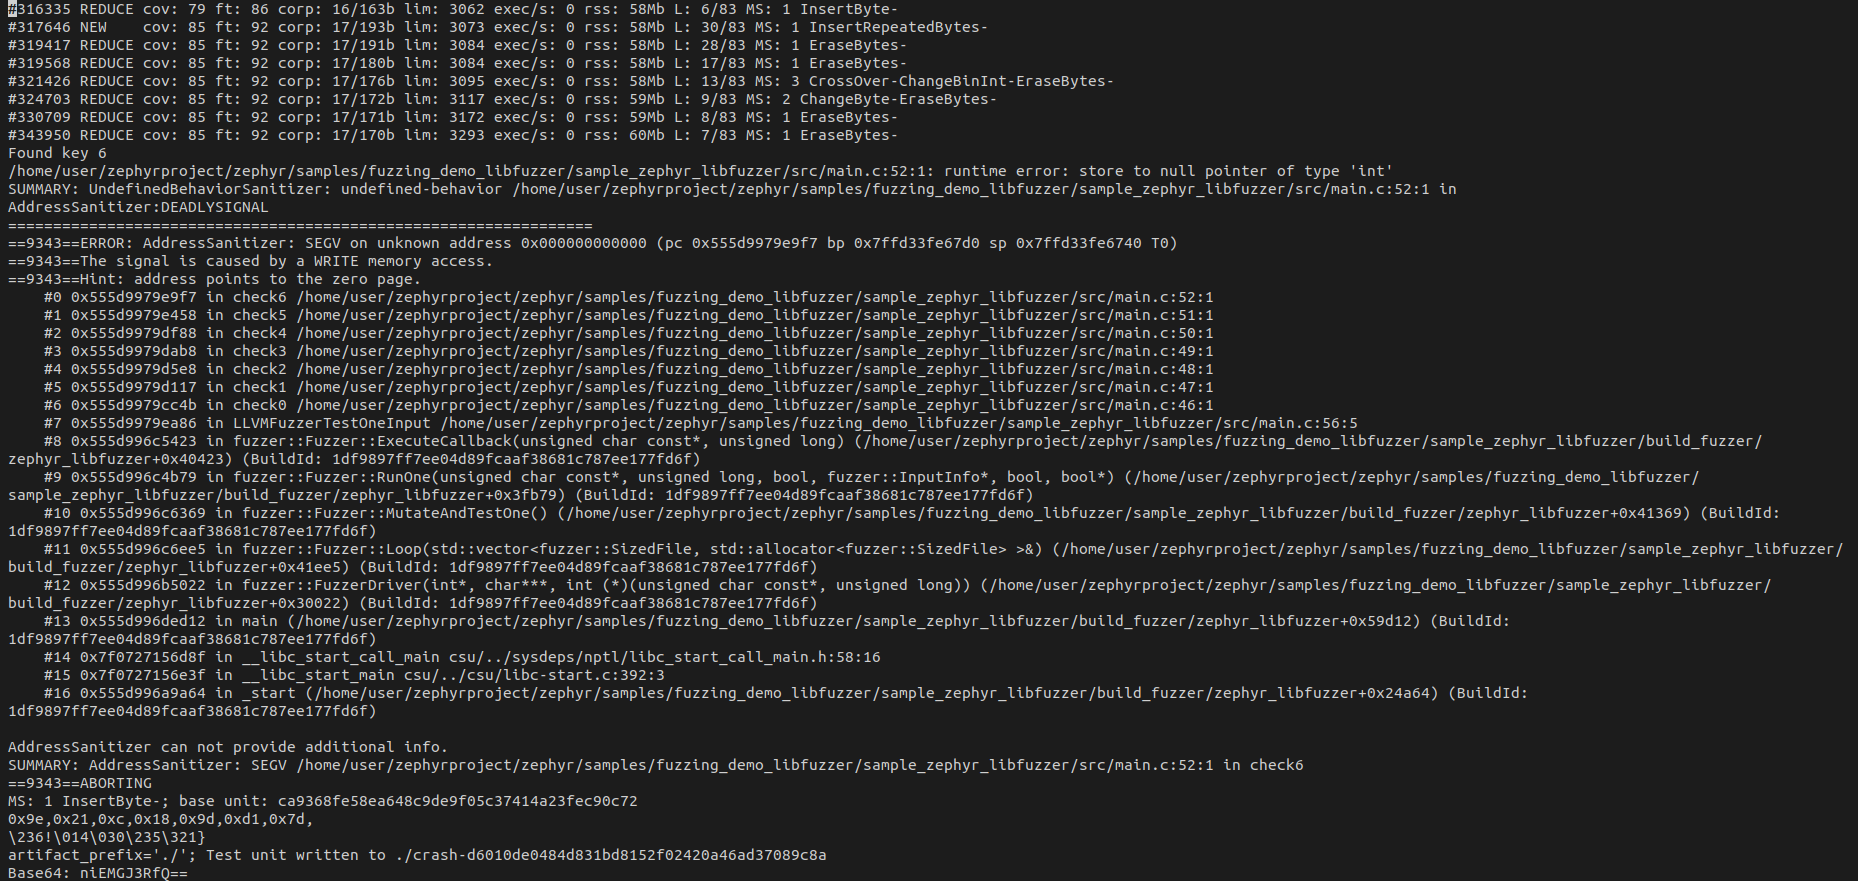
\includegraphics{lib_fuzzer}}
    \caption{AFL++ Execution Screen}\label{fig:lib_fuzzer}
\end{figure}
The fuzzer initialized its execution with a specific random seed,
identified as 758034908\ref{fig:lib_fuzzer}. To reproduce the same
sequence of fuzzing events and outcomes, one may rerun the fuzzer
specifying the argument \texttt{-seed=758034908}.

\begin{minted}[linenos,frame=lines,baselinestretch=1.2,breaklines]{sh}
    INFO: Running with entropic power schedule (0xFF, 100).
    INFO: Seed: 758034908
    INFO: Loaded 1 modules   (157 inline 8-bit counters): 157 [0x555d997e79a8, 0x555d997e7a45), 
    INFO: Loaded 1 PC tables (157 PCs): 157 [0x555d997e7a48,0x555d997e8418),
    INFO: -max_len is not provided; libFuzzer will not generate inputs larger than 4096 bytes
    INFO: A corpus is not provided, starting from an empty corpus
\end{minted}

In its default configuration, \texttt{libFuzzer} operates under
the assumption that the input size is constrained to 4096 bytes or less.
To modify this default input size constraint, two potential strategies exist:
the application of the \texttt{-max\_len=N} argument, where \texttt{N} represents
the desired maximum input length, or the initiation of the fuzzer using a
seed corpus that contains non-empty entries. For this PoC, no corpus or input
is provided, hence the fuzzer starts with an empty corpus.

\begin{minted}[linenos,frame=lines,baselinestretch=1.2,breaklines]{sh}
    #330709 REDUCE cov: 85 ft: 92 corp: 17/171b lim: 3172 exec/s: 0 rss: 59Mb L: 8/83 MS: 1 EraseBytes-
    #343950 REDUCE cov: 85 ft: 92 corp: 17/170b lim: 3293 exec/s: 0 rss: 60Mb L: 7/83 MS: 1 EraseBytes-
    Found key 6
    /home/user/zephyrproject/zephyr/samples/fuzzing_demo_libfuzzer/sample_zephyr_libfuzzer/src/main.c:52:1: runtime error: store to null pointer of type 'int'
    SUMMARY: UndefinedBehaviorSanitizer: undefined-behavior /home/user/zephyrproject/zephyr/samples/fuzzing_demo_libfuzzer/sample_zephyr_libfuzzer/src/main.c:52:1 in
    AddressSanitizer:DEADLYSIGNAL
    =================================================================
    ==9343==ERROR: AddressSanitizer: SEGV on unknown address 0x000000000000 (pc 0x555d9979e9f7 bp 0x7ffd33fe67d0 sp 0x7ffd33fe6740 T0)
    ==9343==The signal is caused by a WRITE memory access.
    ==9343==Hint: address points to the zero page.
\end{minted}

During its execution, \texttt{libFuzzer} has processed a minimum of
316,335(\#330709) distinct inputs. From these, it identified 17 unique
inputs with a combined size of 170 bytes (corpus: 17 entries totaling 170 bytes)
that cumulatively achieve coverage over 85 specific points within the target program.

Remarkably, for one particular input, the integrated \texttt{AddressSanitizer}\cite{GitHubgo55:online}
identified an anomaly characterized as undefined behavior. Consequently, this prompted
the termination of the fuzzer's execution.

Prior to its termination, \texttt{libFuzzer} took the precaution of persisting
the problematic input to the disk, ensuring that the specific circumstances
leading to the anomaly could be independently revisited. To replicate the observed
behavior without engaging in further fuzzing, one can execute the following command:

\begin{minted}[linenos,frame=lines,baselinestretch=1.2,breaklines]{sh}
./zephyr_libfuzzer crash-d6010de0484d831bd8152f02420a46ad37089c8a
\end{minted}

To amalgamate the profiling data, the following command utilizing \texttt{llvm-profdata} can be employed:

\begin{minted}[linenos,frame=lines,baselinestretch=1.2,breaklines]{sh}
llvm-profdata merge -sparse default.profraw -o default.profdata
\end{minted}

This operation produces the files \texttt{default.profraw} and \texttt{default.profdata}, capturing the consolidated profiling information.

For a terminal-based summary of the coverage, the \texttt{llvm-cov} tool provides a report as follows:

\begin{minted}[linenos,frame=lines,baselinestretch=1.2,breaklines]{sh}
llvm-cov report ./zephyr_libfuzzer -instr-profile=default.profdata
\end{minted}

Additionally, to create a more detailed visualization in HTML format, the
subsequent command can be used:

\begin{minted}[linenos,frame=lines,baselinestretch=1.2,breaklines]{sh}
llvm-cov show ./zephyr_libfuzzer -instr-profile=default.profdata -format=html -output-dir=coverage
\end{minted}

This command generates an HTML report, which can be conveniently reviewed in a web browser,
providing an insightful representation of the code's coverage.